\subsection{New Subgrid Methods}
\begin{frame}[t]{Polynomial Decusping}

\begin{itemize}
    \item Rodded 3$\times$3 assembly case used to generate correction factors based on rod position
    \begin{itemize}
        \item One set of calculations performed with refined mesh to eliminate cusping effects
        \item Second set done with coarse mesh
        \item Percent change in \keff{} plotted against percent change in volume fraction for each set of calculations
        \item Difference in curves used to reduce volume fraction during rod homogenization to reduce cusping effects
    \end{itemize}
    \item Sixth order polynomial curves generated for AIC, \bfc{}, and tungsten rods
\end{itemize}

\end{frame}

%%%%%%%%%%%%%%%%%%%%%%%%%%%%%%%%%%%%%%%%%%%%%%%%%%%%%%%%%%%%%%%%%%%%%%%%%%%%%%%%%

\begin{frame}[t]{Polynomial Decusping}
    
\begin{center}
    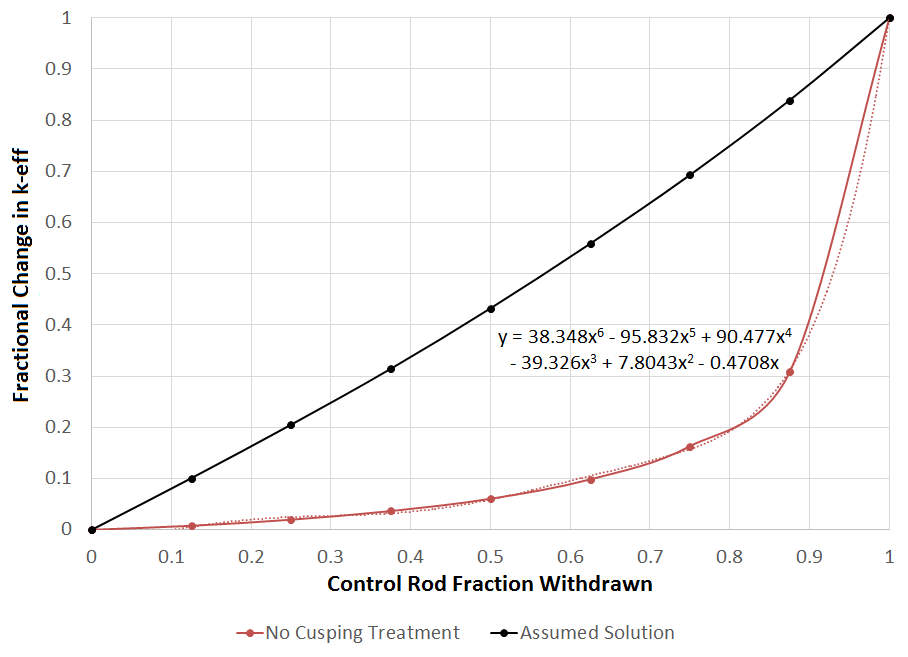
\includegraphics[width=0.8\textwidth]{polynomial_curves.png}
\end{center}
    
\end{frame}

%%%%%%%%%%%%%%%%%%%%%%%%%%%%%%%%%%%%%%%%%%%%%%%%%%%%%%%%%%%%%%%%%%%%%%%%%%%%%%%%%

\begin{frame}[t]{Subplane Collision Probabilities}
    
    \begin{itemize}
        \item Modifications made to subplane scheme \cite{Graham2017Improvementofthe2D/1DMethodUsingtheSub-PlaneScheme,Graham2017RodDecuspingTechniquesforthe2D/1DMethod} to treat axial effects of rod cusping
        \begin{itemize}
            \item Homogenization still uses MOC flux with axial shape factor, but 
            with heterogeneous rodded or unrodded cross sections
            \item Projection rehomogenizes cross sections in partially rodded nodes 
            after CMFD calculation
        \end{itemize}
        \begin{equation}\label{e:nTRACERdecusping}
        \overline{\Sigma_i} = \frac{\phi_{rad,i}^R \phi_{ax,i}^R \Sigma_i^R h^R + \phi_{rad,i}^U \phi_{ax,i}^U \Sigma_i^U h^U}{\phi_{rad,i}^R \phi_{ax,i}^R h^R + \phi_{rad,i}^U \phi_{ax,i}^U h^U} \nonumber
        \end{equation}
    \end{itemize}
    
\end{frame}

%%%%%%%%%%%%%%%%%%%%%%%%%%%%%%%%%%%%%%%%%%%%%%%%%%%%%%%%%%%%%%%%%%%%%%%%%%%%%%%%%

\begin{frame}[t]{Subplane Collision Probabilities}
    
    \begin{columns}
        \begin{column}{0.45\textwidth}
            \begin{itemize}
                \item Sub-plane modifications only capture axial effects
                \begin{itemize}
                    \item MOC uses homogenized cross section
                    \item Radial shape does not accurately reflect either region
                \end{itemize}
                \item 1D collision probabilities (CP) introduced to generate radial 
                shapes
                \begin{itemize}
                    \item Generates radial flux profile for rodded and unrodded region
                    \item Radial profiles used in CMFD homogenization
                    \item Fast calculation
                \end{itemize}
            \end{itemize}
        \end{column}
        \begin{column}{0.55\textwidth}
            \begin{figure}[h]
                \centering
                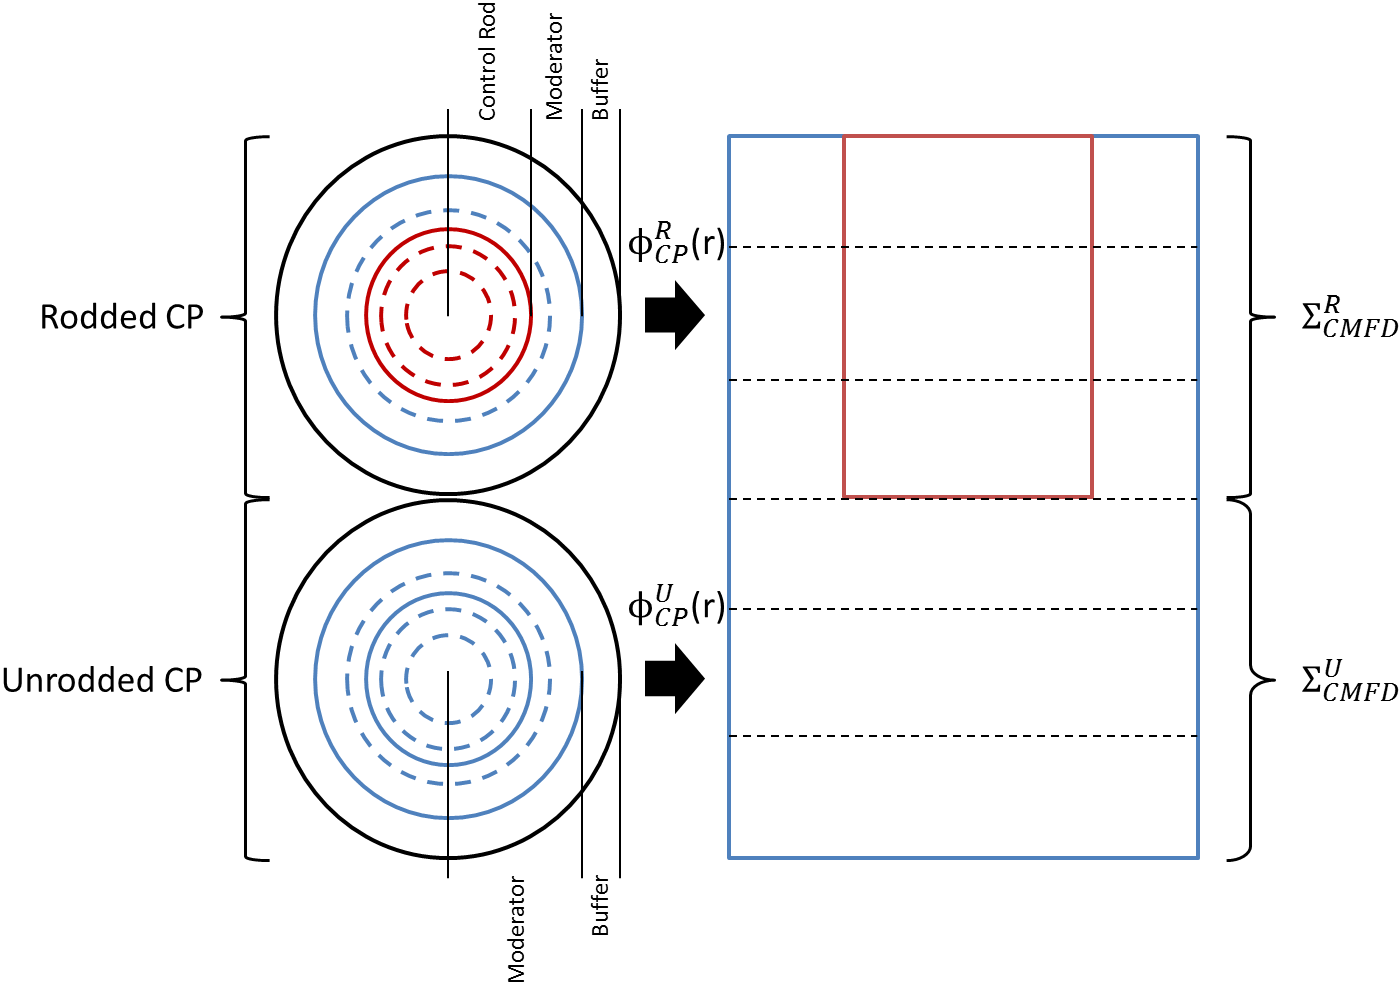
\includegraphics[width=\textwidth]{CPdecusp.png}
            \end{figure}
        \end{column}
    \end{columns}
    
\end{frame}

%%%%%%%%%%%%%%%%%%%%%%%%%%%%%%%%%%%%%%%%%%%%%%%%%%%%%%%%%%%%%%%%%%%%%%%%%%%%%%%%

\begin{frame}[t]{Subray Method of Characteristics}

\begin{itemize}
    \item Other methods do not correctly address the MOC calculation
    \begin{itemize}
        \item Homogenized cross sections are still used for 2D MOC
        \item Flux shape from MOC does not accurately represent rodded or unrodded flux
    \end{itemize}
    \item To improve MOC solutions, heterogeneous cross sections and sources must be accounted for
    \item MOC rays can be split into subrays in the vicinity of partially rodded regions
    \item MOC solution along subrays exponentially converges to $\frac{q}{\Sigma_t}$, allowing subrays to be recombined once axial shape of $q$ flattens sufficiently
\end{itemize}

\end{frame}

%%%%%%%%%%%%%%%%%%%%%%%%%%%%%%%%%%%%%%%%%%%%%%%%%%%%%%%%%%%%%%%%%%%%%%%%%%%%%%%%

\begin{frame}[t]{Subray Method of Characteristics}
    
\begin{center}
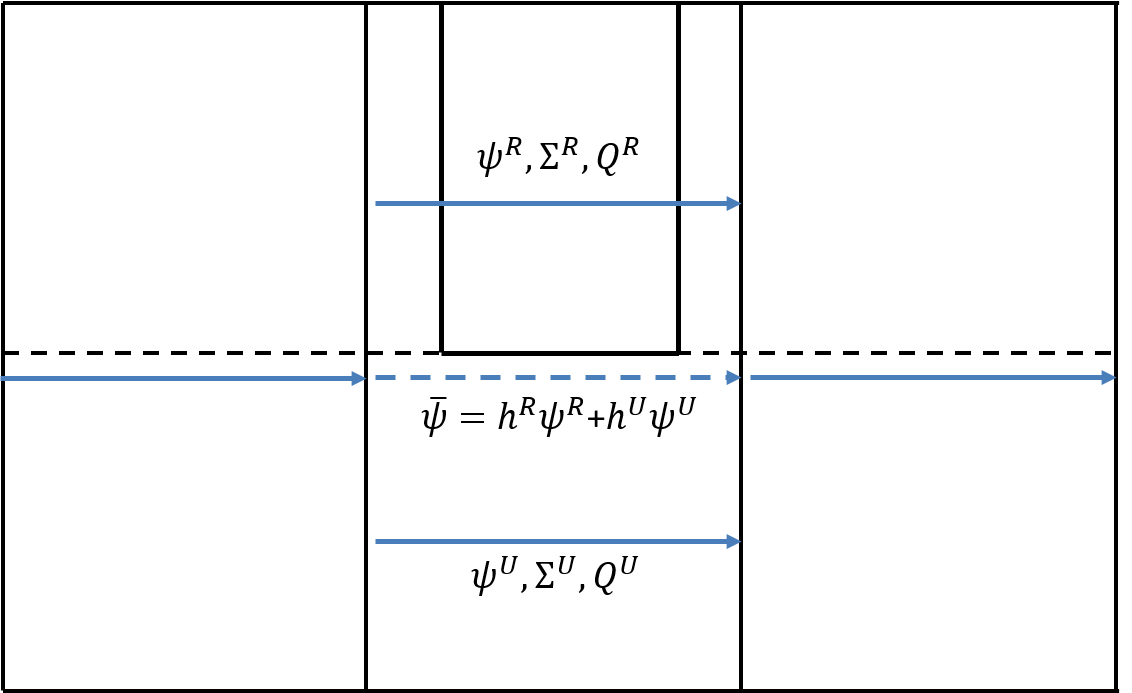
\includegraphics[width=0.8\textwidth]{sub-ray_illustration.png}
\end{center}

\end{frame}

%%%%%%%%%%%%%%%%%%%%%%%%%%%%%%%%%%%%%%%%%%%%%%%%%%%%%%%%%%%%%%%%%%%%%%%%%%%%%%%%

\begin{frame}[t]{Subray Method of Characteristics}
    
    \begin{itemize}
        \item Many modifications were required to enable subray MOC in MPACT:
        \begin{itemize}
            \item Fluxes, cross sections, and sources are stored for subregions that subrays pass through
            \item New MOC sweeper was developed that duplicates long rays using axial volume fractions to average rays together
            \item CMFD projection is used to calculate subregion fluxes and generate subregion sources
            \item Subplane CMFD/P$_3$ results are used to calculate axial TL sources in subregions
            \item Option was added to control how far away from rod subray continues to be used
        \end{itemize}
    \end{itemize}

\end{frame}

%%%%%%%%%%%%%%%%%%%%%%%%%%%%%%%%%%%%%%%%%%%%%%%%%%%%%%%%%%%%%%%%%%%%%%%%%%%%%%%%

\begin{frame}[t]{Subray Method of Characteristics}

\begin{columns}
    \begin{column}{0.5\textwidth}
        \begin{itemize}
            \item Subray is used in the entire pin cell with the partially inserted control rod
            \item To capture farther reaching effects of the rod, subray can also be used in neighboring pin cells:
            \begin{itemize}
                \item Subray-0 (Red)
                \item Subray-1 (Blue)
                \item Subray-2 (Green)
                \item Subray-3 (White)
            \end{itemize}
            \item Calculations become more expensive as more subrays are used, but accuracy should improve
        \end{itemize}
    \end{column}
    \begin{column}{0.5\textwidth}
        \begin{center}
            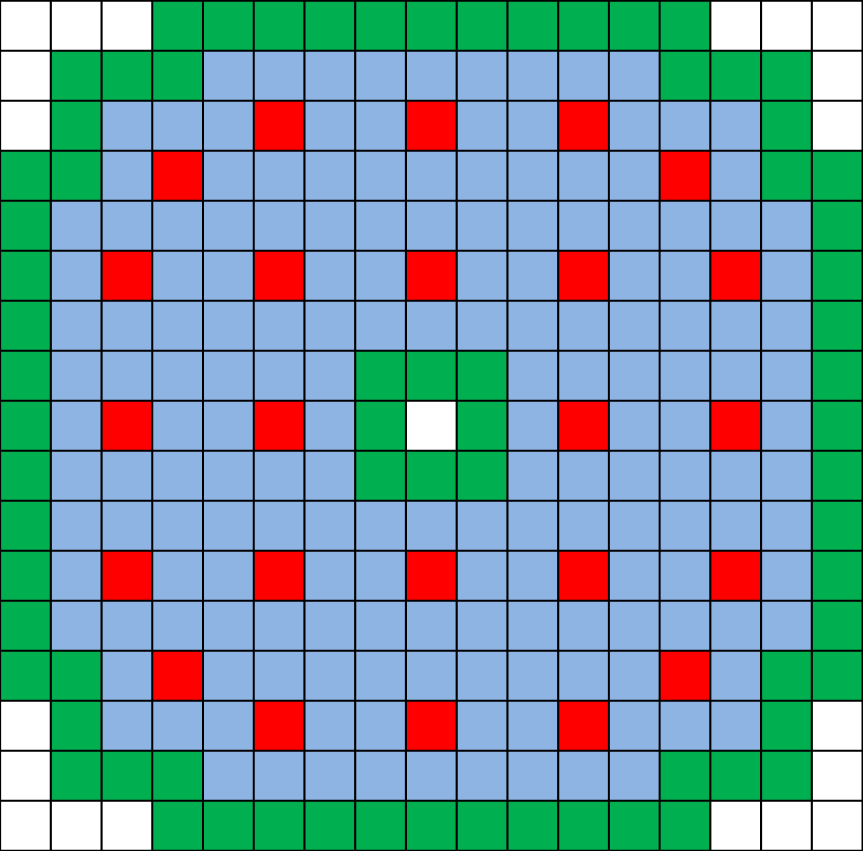
\includegraphics[width=\columnwidth]{recombination.png}
        \end{center}
    \end{column}
\end{columns}

\end{frame}